\begin{enumerate}
    \item Soit $G$ un graphe connexe. Il existe au moins deux composantes connexes dans $G$. Retirer une arête à $G$ revient à retirer une arête à l'une de ces composantes connexes, au risque~:
    \begin{itemize}
        \item ou bien de la diviser en deux nouvelles composantes connexes~;
        \item ou bien de garder autant de composantes connexes.
    \end{itemize}
    Ainsi, il existe au moins autant de composantes connexes à $\Psi(G)$, c'est-à-dire au moins~$2$. D'où $\Psi(G)$ n'est pas connexe.
    \item Si $G$ est acyclique, alors on peut affirmer qu'il manque une ou des arêtes à $G$ pour le rendre cyclique. De fait, en retirer une ne va pas  arranger les choses. $\Psi(G)$ est donc acyclique.
    \item Le graphe $G$ ci-dessous est connexe. Pourtant $\Psi(G)$ ne l'est plus~:\\
    \begin{center}
        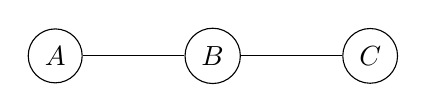
\begin{tikzpicture}[x=2cm, y=2cm]
            \node[draw,circle] (A) at (1,0) {$A$};
            \node[draw,circle] (B) at (2,0) {$B$};
            \node[draw,circle] (C) at (3,0) {$C$};
            \draw (A) -- (B);
            \draw (C) -- (B);
        \end{tikzpicture}
    \end{center}
    \item Le graphe $G$ ci-dessous est cyclique. Pourtant $\Psi(G)$ est acyclique~:\\
    \begin{center}
    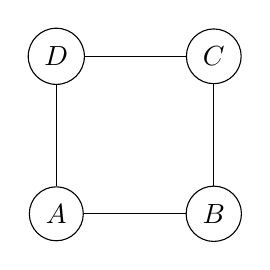
\begin{tikzpicture}[x=2cm, y=2cm]
        \node[draw,circle] (A) at (0,0) {$A$};
        \node[draw,circle] (B) at (1,0) {$B$};
        \node[draw,circle] (C) at (1,1) {$C$};
        \node[draw,circle] (D) at (0,1) {$D$};
        \draw (A) -- (B);
        \draw (C) -- (B);
        \draw (C) -- (D);
        \draw (A) -- (D);
    \end{tikzpicture}
    \end{center}
\end{enumerate}
